In \cite{DBLP:conf/icmt/0001GNEBMPEE14}, Xtext is used for the definition of a source and target satellite procedure language for software translations between both.
In the following we take (abstract) syntax trees of programs written in a programming language $L$ and derivation trees of a context-free grammar defining this language $L$ as synonyms.
We formalise the notion of Xtext EBNF grammars in \cref{def:sec-compl-software-trans:ebnf}, called EBNF grammars with labels.
Labelled elements of the grammar are included in derivation trees whereas unlabelled elements are not. 
In particular, a separation of the terminals in the set $T$ and a family of sets $(C_s)_{s \in S}$ allows a distinction of which terminals are included in derivation trees and which are not.
As software translations aim at the translation of the derivation tree of a program's syntax, this distinction allows to specify which terminals are relevant for the translation and which are not.
The terminals $T$ are not included in derivation trees whereas the elements of the family of sets $(C_s)_{s \in S}$ may be included where each sort $s \in S$ represents a terminal rule in the Xtext grammar and the corresponding carrier set $C_s$ is the set of all words that are derivable from the regular expression of the terminal rule.

\begin{definition}[EBNF Grammar with Labels]
\label{def:sec-compl-software-trans:ebnf}
\index{EBNF grammar!with labels}
An \emph{EBNF grammar $G=(N,n_S,T,L,S,(C_s)_{s \in S},P)$ with labels} is given by
\begin{enumerate}
  \item A set $N$ of non-terminals,
  \item A non-terminal $n_S \in N$ as start symbol,
  \item a set $T$ of terminals,
  \item a set $L$ of labels,
  \item \label{item:sec-compl-software-trans:ebnfA5}a set $S$ of sorts disjoint from the set $N$,
  \item a family of carrier sets $(C_s)_{s \in S}$ with a carrier set $C_s$ for each sort $s \in S$ ($C_s$ defines the terminals for $s$),
  \item a set $P$ of production rules $p\colon n \in N \to R^*$ with a non-terminal $n$ as the left-hand-side (LHS) of the rule and an (empty) sequence $R^*$ as the right-hand-side (RHS) where $R=(L \times N) \cup T \cup (L \times S)$ such that:
  \begin{enumerate}
    \item \label{item:sec-compl-software-trans:ebnfA1}The labelling is unique.
    Thus, let $|p|$ be the amount of label occurrences in production $p$ and $L(p)$ be the set of labels that occur in $p$, then for $P$ it holds that $+_{p \in P} (|p|)=|\cup_{p \in P} (L(p))|$.
    \item \label{item:sec-compl-software-trans:ebnfA2}All labels are used in productions, i.e., $|L|=|\cup_{p \in P} (L(p))|$.
  \end{enumerate} 
    
  The terminals $T$ are called unlabelled whereas $L \times N$ are labelled references to non-terminals $N$ and $L \times S$ are labelled references to sorts $S$ where each sort $s \in S$ represents a set of terminals $C_s$.
  For productions with an empty sequence as RHS we write $n \to \epsilon$, and
  \item \label{item:sec-compl-software-trans:ebnfA8}the start symbol is not target of a reference.
  Therefore, for all productions $p \in P$ with $p\colon n \to R^*$, it holds that $(l,n_s) \in (L \times N)$ does not occur in the RHS $R^*$ of $p$.\envEndMarker
\end{enumerate}
\end{definition}

\cref{def:sec-compl-software-trans:ebnf,item:sec-compl-software-trans:ebnfA5,item:sec-compl-software-trans:ebnfA1,item:sec-compl-software-trans:ebnfA2} enable the definition of the source and target of each labelled reference in an EBNF grammar based on its label $l \in L$ by well-defined functions $s\colon L \to N$ for the source and $t\colon L \to N \cup S$ for the target.

\begin{definition}[Source \& Target of Labels]
\label{def:sec-compl-software-trans:st_labels}
\index{EBNF grammar!with labels!source}
\index{EBNF grammar!with labels!target}
Let $L$ be the labels and $P$ be the productions of an EBNF grammar with labels.
\emph{The source $s\colon L \to N$ of a label $l \in L$} is given by $s(l):=n$ where $(l,n') \in (L \times N)$ occurs in the RHS $R^*$ of a production $p \in P$ with $p\colon n\to R^*$.
\emph{The target $t\colon L \to N \cup S$ of a label $l \in L$} is given by
\begin{center}
$t(l):=\begin{cases}
n' & \quad \text{if } (l,n') \in (L \times N) \text{ occurs in } R^*\\
   & \quad \text{ of a production } p \in P \text{ with } p\colon n \to R^*\\
s  & \quad \text{if } (l,s) \in (L \times S) \text{ occurs in } R^*\\
   & \quad \text{ of a production } p \in P \text{ with } p\colon n \to R^*\\
\end{cases}$
\end{center}
\envEndMarker
\end{definition}

\begin{remark}[Notational Abbreviations]
\label{rem:sec-compl-software-trans:abbr}
In addition to the formal EBNF notation in \cref{def:sec-compl-software-trans:ebnf}, the notation for alternatives in $N \to R_1(R_2|R_3)R_4$ inductively abbreviates the two production rules $N \to R_1R_2R_4$ and $N \to R_1R_3R_4$.
Furthermore, the quantification via the optional operator $?$ in $N \to R_1(R_2)?R_3$ inductively abbreviates the two productions $N \to R_1R_3$ and $N \to R_1R_2R_3$.
\envEndMarker
\end{remark}

\begin{remark}[Context-Free Grammars]
\label{rem:sec-compl-software-trans:ebnf}
Note that \cref{def:sec-compl-software-trans:ebnf} coincides with the classical definition of context-free grammars in two forms.
\begin{enumerate}
  \item \cref{def:sec-compl-software-trans:ebnf} coincides with the classical notion for $T=\varnothing$ and when defining for each terminal $t$ a sort $s_t \in S$ with carrier set $C_{s_t}=\{t\}$ except that an additional unique labelling is required for each occurrence of a non-terminal or sort in the RHS of a production.
  \item \label{item:sec-compl-software-trans:ebnf2}\cref{def:sec-compl-software-trans:ebnf} coincides with the classical notion for $S=\varnothing$.\envEndMarker
\end{enumerate}
For each classical context-free grammar that does not satisfy restriction \cref{def:sec-compl-software-trans:ebnf,item:sec-compl-software-trans:ebnfA8}, the restriction can be bypassed by adding a production to the grammar with a new start symbol as LHS and the old start symbol as RHS without changing the language that is induced by the grammar. 
\end{remark}

\begin{example}[EBNF Grammar with Labels]
\label{ex:sec-compl-software-trans:ebnf}
Each line in lines 1-17 of the EBNF grammar in \cref{sec-compl-software-trans-tgg,ex:sec-compl-software-trans:xtext_ebnf} represents a grammar rule of the form LHS:RHS where the LHS of the rule consists of exactly one non-terminal and the RHS is a sequence of unlabelled terminals and labelled references to non-terminals or sorts.
For example, in line 4, \textsf{class},\textsf{':'},\textsf{\{} and \textsf{\}} are unlabelled terminals whereas \textsf{attr1=ATTR} is a reference to non-terminal \textsf{ATTR} with label \textsf{attr1} and \textsf{name1=STRING} is a reference to sort \textsf{STRING} with label \textsf{name1}.
The sorts are given by Xtext terminal rules in lines 20-23.

Based on \cref{def:sec-compl-software-trans:ebnf}, the formal definition of the grammar is given by:

\begin{enumerate}
  \item The set $N$ of non-terminals that are given by the LHSs of the grammar rules with $N=\{PROGRAM,CL\_LST,CLASS,STR\_LST,ATTR,$ $NEW,ACCESS,ST\_LST,ST,ASG,PRINT,$ $READ,IF,COND,GOTO\}$,
  \item the first rule $PROGRAM$ as start symbol,
  \item the set $T$ of terminals that are given by the words enclosed by quotes in the RHSs of the rules with $T=\{\texttt{\textbackslash n},class,:,\{,\},,,;,new,.,=,print,read,if,then,end,!=,goto\}$,
  \item the set $L$ of labels that are given by the names of the references in the RHSs of the rules with $L=\{first,cl1,n1,n2,name1,e,attr1,name2,n3,type,$ $name3,n4,cl2,obj,attr2,st,n5,a,p,r,i,g,a1,a2,a3,$ $a4,a5,out,in1,in2,c,body,l,r1,r2,r3,line\}$,
  \item the sorts that are given by the terminal rules with $S=\{NULL,STRING,VAR,INT\}$,
  \item the carrier sets that are given by the sets of all words that are derivable from the regular expressions of the corresponding terminal rules with $C_{STRING}=\{w \mid w \text{ is derivable from '"'} .^* \text{'"'}\}$, $C_{VAR}=\{w \mid w \text{ is derivable from } ('a'..'z'|'A'..'Z')+\}$, $C_{INT}=\{w \mid w \text{ is derivable from } (0..9)+\}$ and $C_{NULL}=\{null\}$, and
  \item the following productions by considering the notational abbreviations in \cref{rem:sec-compl-software-trans:abbr}:
  \begin{enumerate}
    \item[a)] $PROGRAM \to (first,CL\_LST)$,
    \item[b)] $CL\_LST \to (cl1,CLASS)$,
    \item[c)] $CL\_LST \to (cl1,CLASS)\ \texttt{\textbackslash n}\ (n1,CL\_LST)$,
    \item[d)] $CL\_LST \to (cl1,CLASS)\ \texttt{\textbackslash n}\ (n2,ST\_LST)$,
    \item[e)] $CLASS \to class\ (name1,STRING)\ \{\ \}$,
    \item[f)] $CLASS \to class\ (name1,STRING)\ $ $\{\ (attr1,ATTR)\ \}$,
    \item[g)] $CLASS \to class\ (name1,STRING)\ :\ (e,STR\_LST)\ \{\ \}$,
    \item[h)] $CLASS \to class\ (name1,STRING)\ :\ (e,STR\_LST)\ \{\ (attr1,ATTR)\ \}$,
    \item[i)] $STR\_LST \to (name2,STRING)$,
    \item[j)] $STR\_LST \to (name2,STRING)$ $\ ,\ (n3,STR\_LST)$,
    \item[k)] $ATTR \to (type,STRING)\ (name3,STRING)\ ;$,
    \item[l)] $ATTR \to (type,STRING)\ (name3,STRING)\ ;$ $\ (n4,ATTR)$, and
    \item[m)] the productions for the rules in lines 8 to 17 are defined analogously.
%     \item[a)] $ST\_LST \to (s,ST)\ ;$,
%     \item[b)] $ST\_LST \to (s,ST)\ ;\ n\ (next,ST\_LST)$,
%     \item[c)] $ST \to (i,IF)$,
%     \item[d)] $ST \to (p,PRINT)$,
%     \item[e)] $ST \to (r,READ)$,
%     \item[f)] $PRINT \to print\ (out,STRING)$,
%     \item[g)] $READ \to read\ (in,VAR)$,
%     \item[h)] $IF \to if\ <\ (c,COND)\ >\ then\ (body,ST)$, and
%     \item[i)] $COND \to (left,VAR)\ =\ (right,STRING)$.
  \end{enumerate}
\end{enumerate}
Note that the set $S$ of sorts is disjoint from the set $N$ of non-terminals, the labelling is unique and all labels are used in productions (cf. \cref{def:sec-compl-software-trans:ebnf,item:sec-compl-software-trans:ebnfA1,item:sec-compl-software-trans:ebnfA2}).
This allows the definition of the source and target of label \textsf{name1} with $s(name1)=CLASS$ and $t(name1)=STRING$ (cf. \cref{def:sec-compl-software-trans:st_labels}).
The sources and targets of the other labels are given analogously.
Furthermore, the start symbol is not target of a reference (cf. \cref{def:sec-compl-software-trans:ebnf,item:sec-compl-software-trans:ebnfA8}).
\envEndMarker
\end{example}

Software translations are performed by translating derivation trees of programs that are induced by the underlying grammar of the programming language to models of the target language.
\cref{def:sec-compl-software-trans:lang_der} defines the language of derivation trees that are induced by an EBNF grammar.
The root node of each derivation tree is the start symbol of the grammar, the internal nodes are non-terminals whereas the leafs are non-terminals or terminals $(C_s)_{s \in S}$ of sorts $S$.
Note that by \cref{def:sec-compl-software-trans:lang_der,item:sec-compl-software-trans:lang_der2}, terminals $T$ of the grammar are not contained in derivation trees making them to a special type of abstract syntax trees of programs where not all details of a grammar are reflected in the trees (cf. concrete syntax trees).

\begin{definition}[Language of Derivation Trees]
\label{def:sec-compl-software-trans:lang_der}
\index{language!of derivation trees}
Let $G=(N,n_s,T,L,S,(C_s)_{s \in S},P)$ be an EBNF grammar with labels.
Then, \emph{the language $\Der(G):=trees(n_S)$ of derivation trees of $G$} is inductively defined by all trees $trees(n_S)$ with root node $n_S$ and:
\begin{enumerate}
  \item $trees(\epsilon)=\{\epsilon\}$,
  \item \label{item:sec-compl-software-trans:lang_der2}$trees(t \in T)=\{\epsilon\}$,
  \item $trees((l,s) \in (L \times S))=\cup_{t \in C_s}\{(l,t)\}$,
  \item $trees((l,n) \in (L \times N))=\cup_{m \in trees(n)}\{(l,m)\}$, and
  \item $trees(n \in N)=\cup_{p \in P'}trees(r_n) \circ \ldots \circ trees(r_1) \circ \{n\}$, for $p\colon n \to r_1 \ldots r_n$ and $P \supseteq P'=\{p\colon n \to R^* \mid p \in P \text{ for some arbitrary }R^*\}$.\envEndMarker 
\end{enumerate}
\end{definition}

\begin{example}[Derivation Tree]
\label{ex:sec-compl-software-trans:der_tree}
Below, the derivation tree of the program in \cref{sec-compl-software-trans-tgg,ex:sec-compl-software-trans:prog} up to line 3 is presented in formal notation by following \cref{def:sec-compl-software-trans:lang_der}.
The corresponding visual graph-like notation is presented in \cref{sec-compl-software-trans-tgg,ex:sec-compl-software-trans:der_tree1}.
 
\begin{lstlisting}[frame=none,language=pseudocode]
PROGRAM (first, CL_LST (cl1, CLASS (name1, "Person") (attr1, ATTR (type, "String") (name3, "name") (n4, ATTR (type, "Person") (name3, "next")))) (n1, CL_LST (cl1, CLASS (name1, "Employee") (e, STR_LST (name2, "Person")) (attr1, ATTR (type, "String) (name3, "salary"))) (n2, ...)))
\end{lstlisting}

The complete tree that covers the whole program is given analogously.
Note that the keywords of the language (terminals $T$ of the grammar) are not contained in the tree.
\envEndMarker
\end{example}

\begin{remark}[Visual Notation of Graphs]
\label{rem:sec-compl-software-trans:vis_graphs}
Note that the graphs in \cref{ex:sec-compl-software-trans:der_tree} are presented in visual notation.
The type of each node and edge is indicated by a preceeding colon.
Thus, the notation \textsf{:n} means that the node or edge is of type $n$.
Technically, the typing of a node (edge) \textsf{:n} is given by a mapping from that node (edge) to node (edge) $n$ in the type graph along the given type morphism of the typed graph containing this node (edge) (cf. \cref{def:sec-compl-software-trans:ebnf_typegraph}).
Furthermore, for node attributes we do not use the explicit E-graph notation but visualise them directly with attribute name and value inside the corresponding nodes.
\envEndMarker
\end{remark}

\begin{remark}[Language of Derivation Trees]
In \cref{def:sec-compl-software-trans:lang_der}, operation $\circ$ is the concatenation of words with $\epsilon$ being the empty word, i.e., $w \circ \epsilon=\epsilon \circ w=w$ for all words $w$.
The concatenation of sets of words $W' \circ W=\{w' \circ w \mid w \in W, w' \in W'\}$ is given by all possible concatenations of words.
Note that \cref{def:sec-compl-software-trans:lang_der} does not coincide with the classical notion of derivation trees (concrete syntax trees) of context-free grammars, not even if \cref{rem:sec-compl-software-trans:ebnf,item:sec-compl-software-trans:ebnf2} is assumed, since, terminals $T$ are not represented in the trees.
\envEndMarker
\end{remark}

\begin{remark}[Decidability of Derivation Tree Translations]
Note that the context-free language $\{a^nb^n \mid n \in \mathcal{N}\}$ of words with an equal amount of $a$'s and $b$'s that is given by a context-free grammar $G$ with one production $p$ (given below) may induce a regular language $\Lang(G)$ of derivation trees by following \cref{def:sec-compl-software-trans:lang_der} (cf. regular structure of derivation trees below).
However, as the graph grammar $\GG$ for describing the translation of derivation trees may be context-free, the inclusion problem $\Lang(G) \subseteq \Lang(\GG)$ remains undecidable, in general.
\begin{center}
$p\colon S \to a\ s=S\ b$\newline
Derivation trees: \textsf{S (s, S (s, \ldots))}\newline
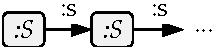
\includegraphics[width=.2\textwidth]{img/software_trans/ast2.pdf}
\end{center}
\envEndMarker
\end{remark}

In order to close the gap between word grammars and the theory of graph transformations, we introduce a mapping from derivation trees as defined in \cref{def:sec-compl-software-trans:lang_der} to typed attributed graphs.
The graph language of derivation trees is given by an attributed type graph together with a set of graph constraints.
Thus, the mapping is based on the coding of EBNF grammars with labels to attributed type graphs, called EBNF type graphs, together with graph contraints, called EBNF graph constraints, such that the language of derivation trees that is induced by the EBNF grammar is equivalent to the language of graphs that are typed over the type graph and that fulfill the constraints.
This enables the application of model transformations based on triple graph grammars to translate the derivation trees.
Furthermore, this enables the application of the developed theory of domain completeness in order to verify the completeness of the translation.

\cref{def:sec-compl-software-trans:ebnf_typegraph} defines the coding of EBNF grammars from \cref{def:sec-compl-software-trans:ebnf} to EBNF type graphs (cf. Def. 8.7 in \cite{Ehrig:2006:FAG:1121741}) and \cref{def:sec-compl-software-trans:ebnf_constraints} to EBNF graph constraints.
The coding to EBNF type graphs is performed as follows.

\begin{enumerate}
  \item Each non-terminal $n$ is represented by a node $n$.
  \item \label{item:sec-compl-software-trans:tg1}Each reference $(l,n')$ with label $l$ to a non-terminal $n'$ in the RHS of a production $n \to R^*$ is represented by an edge $l$ from node $n$ to $n'$.
  \item \label{item:sec-compl-software-trans:tg2}Each reference $(l,s)$ with label $l$ to a sort $s$ in the RHS of a production $n \to R^*$ is represented by an attribute $l$ of node $n$ and of type $s$.
\end{enumerate}

The requirement in \cref{def:sec-compl-software-trans:ebnf,item:sec-compl-software-trans:ebnfA5} that the non-terminals $N$ are disjoint from the set of sorts $S$ simplifies the destinction between the labels that become edges and those labels that become node attributes in the type graph in \cref{item:sec-compl-software-trans:tg1,item:sec-compl-software-trans:tg2} and \cref{def:sec-compl-software-trans:ebnf_typegraph,item:sec-compl-software-trans:ebnf_typegraph3,item:sec-compl-software-trans:ebnf_typegraph4}.

\begin{definition}[EBNF Type Graph]
\label{def:sec-compl-software-trans:ebnf_typegraph}
\index{type graph!EBNF type graph}
Given an EBNF grammar with labels $G=(N,n_s,T,L,S,(C_s)_{s \in S},P)$.
\emph{The type graph $\TG_G^{DSIG}=(\TG,Z)$ of $G$} is given by
\begin{enumerate}
  \item an algebraic data signature $DSIG=(S,OP)$ with sorts $S$ and an arbitrary set of operations $OP$,
  \item the final $DSIG$-algebra $Z=((Z_s)_{s \in S},OP_Z)$ with $Z_s=\{s\}$ for each $s \in S$, and
  \item an E-graph $\TG=(V_{\TG}$ $,V_D,E_{\TG},E_{NA},E_{EA}$ $,(source_j,target_j)_{j \in \{\TG,NA,EA\}})$ with
  \begin{enumerate}
    \item $V_{\TG}=N$,
    \item $V_D=\cup_{s \in S}Z_s$,
    \item \label{item:sec-compl-software-trans:ebnf_typegraph3}$E_{\TG}=\{l \mid l \in L, t(l) \in N\}$,
    \item \label{item:sec-compl-software-trans:ebnf_typegraph4}$E_{NA}=\{l \mid l \in L, t(l) \in S\}$,
    \item $E_{EA}=\varnothing$,
    \item $source_j\colon E_j \to V_\TG$ with $source_j(e):=s(e)$,
    \item $target_\TG\colon E_\TG \to V_\TG$ with $target_\TG(e):=t(e)$, and
    \item $target_{NA}\colon E_{NA} \to V_D$ with $target_{NA}(e):=t(e)$ where $\{t(e)\} = Z_{t(e)}$.
  \end{enumerate}
\end{enumerate}
For the definitions of $s(L)$ and $t(L)$ we refer to \cref{def:sec-compl-software-trans:st_labels}.
\envEndMarker
\end{definition}

\begin{example}[EBNF Type Graph]
\label{ex:sec-compl-software-trans-mapping:ebnf_tg}
The EBNF type graph of the grammar in \cref{ex:sec-compl-software-trans:ebnf} is given below.
The type graph represents the structure of the grammar where
\begin{enumerate}
  \item all non-terminals $N$ of the grammar become nodes in the graph (e.g., non-terminal $PRINT$ becomes node \textsf{PRINT}),
  \item all labelled references to non-terminals in the grammar become edges in the graph with corresponding non-terminals nodes as source and target (e.g., labelled reference $(cl1,CLASS)$ in productions $CL\_LST\to \ldots$ becomes edge \textsf{cl1} with source node \textsf{CL\_LST} and target node \textsf{CLASS}), and
  \item all labelled references to sorts in the grammar become attributes of corresponding non-terminal nodes in the graph.
  Furthermore, the type of each attribute is given by the corresponding referrenced sort (e.g., labelled reference $(name1,STRING)$ in productions $CLASS \to \ldots$ becomes attribute \textsf{name1} of node \textsf{CLASS} with type \textsf{STRING}).
\end{enumerate}
By \cref{def:sec-compl-software-trans:ebnf_typegraph}, the formal notation of the EBNF type graph from above is given as follows:
\begin{enumerate}
  \item $S=\{STRING,VAR,INT,NULL\}$,
  \item $Z=((Z_s)_{s \in S},OP_Z)$ with $Z_s=\{s\}$,
  \item \begin{enumerate}
    \item $V_\TG=N$,
    \item $V_D=\{STRING,VAR,INT,NULL\}$,
    \item $E_\TG=\{first,n1,n2,n3,n4,n5,cl1,e,attr1,body,$ $st,a,p,r,i,g,a2,a4,a5,out,in2,c,r2\}$,
    \item $E_{NA}=\{name1,name2,name,type,line,a1,a3,$ $cl2,in1,obj,attr2,l,r1,r3\}$,
    \item $source_\TG(n1)=source_\TG(n2)=source_\TG(cl1)=$ $CL\_LST$ for edges $n1,n2,cl1$ and $source_{NA}(name3)=source_{NA}(type)=ATTR$ for node attributes $name,type$, and
    \item $target_\TG(n2)=target_\TG(n5)=$ $target_\TG(body)=ST\_LST$ for edges $n2,n5,body$ and $target_{NA}(name3)=target_{NA}(type)=STRING$ for node attributes $name,type$ (the sources and targets of the other edges and node attributes are given analogously).\envEndMarker
  \end{enumerate}
\end{enumerate}
The visual notation of the EBNF type graph is given by the elements in (Root + Statements + Classes) in \cref{sec-compl-software-trans-tgg,fig:sec-compl-software-trans:tg_ebnf}.
\end{example}

In order that all graphs typed over an EBNF type graph are actually graph representations of an EBNF grammar's derivation tree, the graphs additionally need to be restricted to obtain tree-structures.
These restrictions are expressed by EBNF graph constraints which are derived from the EBNF grammar.
While the EBNF type graph defines the overall structure of the EBNF grammar and the domains of labelled terminals, the EBNF graph constraints ensure that the syntax graphs are actually trees and represent the grammar structure, i.e.,
\begin{enumerate}
  \item For the start symbol of the EBNF grammar there exists exactly one root node with no incoming edge,
  \item for each grammar production rule there exists exactly one node with at least one outgoing and incoming edge for each edge type, and
  \item each syntax graph has no cycles.
\end{enumerate}
The graph constraints are defined based on the notion of graphs over a set of labels.
Given a set of labels $L$ such that all labels in $L$ have the same source $n$, then the graph over $L$ is given by a node \textsf{:n} of type $n$ together with an edge for each label with \textsf{:n} as source node and the target of the label as type of the dedicated target node.
Labels with non-terminals as targets become graph edges whereas labels with sorts as targets become node attribute edges in the graph with unique variables as attribute values (cf. \cref{ex:sec-compl-software-trans:graph_set_labels}).

\begin{definition}[Graph over a set of Labels]
\label{def:sec-compl-software-trans:gr_labels}
\index{graph!over labels}
Given an EBNF grammar with labels $G=(N,n_s,T,L,S,(C_s)_{s \in S},P)$ and the corresponding EBNF type graph $\TG_G^{DSIG}$.
Let $E \in \mathcal{P}(L)$ be a set of labels with same source $n$, i.e., for all labels $e_1,e_2 \in E$ it is true that $s(e_1)=s(e_2)=n$ (cf. \cref{def:sec-compl-software-trans:st_labels}). 
A \emph{graph over a set of labels} $E$ is given by an attributed graph $G_E=(G,T_{DSIG}((X_s)_{s \in S}))$
\begin{enumerate}
  \item that is typed over $\TG_G^{DSIG}$,
  \item with $DSIG$-term-algebra $T_{DSIG}((X_s)_{s \in S})$ with an infinite, countable set $X_s=\{x_i\mid i \in \mathbb{N}\}$ of variables for each sort $s$, and
  \item with graph $G=G(E,n,1)$ which is composed as follows based on graphs $R_n,R_e$ and $R_{e,i}$ in \cref{fig:sec-compl-software-trans:gcs} 2).
	\begin{center}
	$G(E,n,i):=\begin{cases}
	R_n & \quad \text{if } E=\varnothing,\\
	R_e +_{R_{s(e)}} G(E \setminus e,s(e),i) & \quad \text{if } t(e) \in N,\\
	R_{e,i} +_{R_{s(e)}} G(E \setminus e,s(e),i+1) & \quad \text{if } t(e) \in S\\
	\end{cases}$
	\end{center}  
\end{enumerate}
\envEndMarker
\end{definition}

\begin{remark}[Uniqueness of Graphs over Labels]
Note that the construction in \cref{def:sec-compl-software-trans:gr_labels} may lead to a set $S$ of different graphs for a given set of labels $E$, since, the selection of labels during the construction is non-determinstic which may lead to different variables as node attribute values.
However, $S$ is an isomorphism class, i.e., all graphs in $S$ are unique up to isomorphisms, and technically \cref{def:sec-compl-software-trans:gr_labels} is defined based on representatives of these classes only.
\envEndMarker
\end{remark}

\begin{remark}[Visual Notation of Graph Morphisms]
By $A +_I B$, we denote the gluing of graphs $A$ and $B$ over a common interface graph $I$.
Technically, the gluing is given by a pushout over morphisms $I \to A$ and $I \to B$.
The morphisms for the recursive gluing of graphs in \cref{def:sec-compl-software-trans:gr_labels} are given by the names of the nodes and edges in the graphs.
Thus, in addition to \cref{rem:sec-compl-software-trans:vis_graphs}, nodes and edges may have names.
Names are written before the colon.
Thus, the notation \textsf{1:n} means that the node or edge has the name $1$.
For a morphism $I \to A$ between two arbitrary graphs $I$ and $A$, the names are used to indicate the mappings along the morphism.
For example in \cref{fig:sec-compl-software-trans:gcs}, node \textsf{1:n} in graph $R_n$ is explicitly mapped to the source node \textsf{1:n} of edge \text{:e} in graph $R_e$ along morphism $R_n \to R_e$ and is not mapped to node \textsf{:t(e)} which would also be possible for $t(e)=n$ but is not intended, as, this would change the desired semantics of the EBNF graph constraints in \cref{def:sec-compl-software-trans:ebnf_constraints,item:sec-compl-software-trans:ebnf_constraints2}.
Furthermore in contrast to \cref{rem:sec-compl-software-trans:vis_graphs}, for node attributes in graphs of EBNF graph constraints we use the explicit E-graph notation in \cref{def:sec-compl-software-trans:ebnf_constraints}, i.e., node attributes are explicit edges from the corresponding node to an explicit data node as attribute value.
\envEndMarker
\end{remark}

\begin{example}[Graph over a set of Labels]
\label{ex:sec-compl-software-trans:graph_set_labels}
Given the set of labels $L=\{a_1,\ldots,a_n,b_1,\ldots,b_m\}$ where all labels have the same source ($n=s(a_1)=\ldots=s(a_n)=s(b_1)=\ldots=s(b_m)$), the targets of $a_1,\ldots,a_n$ are non-terminals ($t(a_1),\ldots,t(a_n) \in N$) and the targets of $b_1,\ldots,b_m$ are sorts ($t(b_1),\ldots,t(b_m) \in S$).
Then, the graph over $L$ is as follows.
\begin{center}
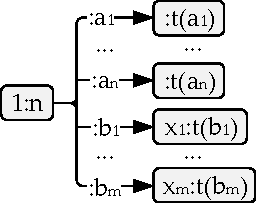
\includegraphics[width=.23\textwidth]{img/software_trans/gr_labels.pdf}
\end{center}
Note that the node attribute values $(x_i)_{i \in \{1,\ldots,m\}}$ are ensured to be unique by construction \cref{def:sec-compl-software-trans:gr_labels}, i.e., there does not exist two different attributes $b_j,b_k$ with $j,k \in \{1,\ldots,m\},j \neq k$ of node \textsf{1:n} having the same variable $x_i$ as value in the graph.
\envEndMarker
\end{example}

\begin{remark}[Subsets of Labels \& Induced Morphisms]
\label{rem:sec-compl-software-trans:subset_labels_mor}
Given a set of labels $L$ and a subset $L' \subseteq L$.
Furthermore, let $G_L$ be a graph over $L$ and $G_{L'}$ a graph over $L'$.
If $L'$ is non-empty, then there exists a unique morphism $G_{L'} \to G_L$ that is induced by the labels, since, each label becomes an unique edge with a unique edge type in graphs $G_L$ and $G_{L'}$ by \cref{def:sec-compl-software-trans:ebnf_typegraph,def:sec-compl-software-trans:gr_labels}, and morphisms are type preserving, i.e., nodes and edges in one graph must be mapped to nodes and edges of the same type in the other graph along morphisms.
\envEndMarker
\end{remark}

\begin{figure*}[!tb]
\centering
\begin{tabular}{c|c}
  \begin{tabular}[t]{lll}
  $R_1$ & $=$ & \raisebox{-.25\height}{
\includegraphics[height=.5cm]{img/software_trans/c1.pdf}}, \\ \\
  $R_2$ & $=$ & \raisebox{-.25\height}{
\includegraphics[height=.5cm]{img/software_trans/c2.pdf}}, and \\ \\
  $R_e$ & $=$ & \raisebox{-.25\height}{
\includegraphics[height=.5cm]{img/software_trans/c3.pdf}}
  \end{tabular} &
  \begin{tabular}[t]{lll}
  $R_n$ & $=$ & \raisebox{-.25\height}{
\includegraphics[height=.5cm]{img/software_trans/c5.pdf}}, \\ \\
  $R_e$ & $=$ & \raisebox{-.25\height}{
\includegraphics[height=.5cm]{img/software_trans/c6.pdf}}, and \\ \\
  $R_{e,i}$ & $=$ & \raisebox{-.25\height}{
\includegraphics[height=.5cm]{img/software_trans/c7.pdf}} with \\
  & & $x_i \in X_{t(e)}$ being a variable \\
  & & of sort $t(e)$.
  \end{tabular} \\
  \textbf{1)} & \textbf{2)} \\
  \multicolumn{2}{c}{\begin{tabular}[t]{lll}
  $R_e$ & $=$ & \raisebox{-.5\height}{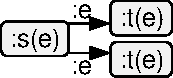
\includegraphics[height=1.1cm]{img/software_trans/c8.pdf}}, \\ \\
  $R_{e1,e2}$ & $=$ & \raisebox{-.25\height}{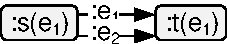
\includegraphics[height=.63cm]{img/software_trans/c9.pdf}}, \\ \\
  $\underline{R}_{e1,e2}$ & $=$ & \raisebox{-.45\height}{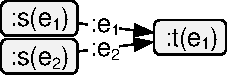
\includegraphics[height=1.05cm]{img/software_trans/c10.pdf}}, and \\ \\
  $R_r$ & $=$ & \raisebox{-.25\height}{
\includegraphics[height=.5cm]{img/software_trans/c4.pdf}}
  \end{tabular}} \\
  \multicolumn{2}{c}{\textbf{3)}}
\end{tabular}
\caption{Visual notation of graphs for graph constraints in \cref{def:sec-compl-software-trans:ebnf_constraints}}
\label{fig:sec-compl-software-trans:gcs}
\end{figure*}

The set of EBNF graph constraints w.r.t. an EBNF grammar is the union of three sets $C_{Root},C_{Ref},C_{Mul}$ of local constraints and a set $\ol{C}_G$ of global constraints.
\cref{def:sec-compl-software-trans:ebnf,item:sec-compl-software-trans:ebnfA8} simplifies the definition of the set of EBNF graph constraints, as, this rectriction allows the unique denotation of the root node of each tree-like graph.

\begin{definition}[EBNF Graph Constraints]
\label{def:sec-compl-software-trans:ebnf_constraints}
\index{graph constraint!EBNF graph constraints}
Given an EBNF grammar with labels $G=(N,n_s,T,L,S,(C_s)_{s \in S},P)$ and the corresponding EBNF type graph $\TG_G^{DSIG}$.
\emph{The set of EBNF graph constraints $C_G$ w.r.t. $G$} are given by sub-sets $C_G=C_{Root} \cup C_{Ref} \cup C_{Mul} \cup \ol{C}_G$ of graph constraints that are typed over $\TG_G^{DSIG}$ and share the same $DSIG$-term-algebra $T_{DSIG}((X_s)_{s \in S})$ with an infinite, countable set $X_s=\{x_i\mid i \in \mathbb{N}\}$ of variables for each sort $s$.
The sub-sets are defined as follows based on the graphs in \cref{fig:sec-compl-software-trans:gcs}.
\begin{enumerate}
  \item $C_{Root}=C_1 \cup C_2 \cup C_3$ with
  \begin{enumerate}
    \item $C_1=\{\exists(\varnothing \to R_1, \true)\}$,
    \item $C_2=\{\neg\exists(\varnothing \to R_2, \true)\}$, and
    \item $C_3=\{\neg\exists(\varnothing \to R_e, \true) \mid e \in L,t(e)=n_s\}$,
  \end{enumerate}
  \item \label{item:sec-compl-software-trans:ebnf_constraints2}
  $C_{Ref}=C_1 \cup C_2 \cup C_3$ with
  \begin{enumerate}
    \item For $n \in N$, with $P_n=\{p \mid p \in P,p \text{ is of form }p\colon n \to R^*\}$ we denote the set of productions with non-terminal $n$ as LHS.
  	Furthermore, for production $p \in P_n$, with $E_p=\{e \mid e \in L, (e,\_) \text{ occurs in RHS }R^*\text{ of }p\}$ we denote the set of labels that occur in $p$ with same source $n$ and therefore must exist for each occurrence of $n$ in a graph.
  
  	$C_1=\{\forall(\varnothing \to R_n,\vee_{p \in P_n}(\exists(R_n \to G_{E_p},\true))) \mid n \in N\}$ with $G_{E_p}$ being the graph over $E_p$ (cf. \cref{def:sec-compl-software-trans:gr_labels}) and $R_n \to G_{E_p}$ being the morphism as induced by the node names of the graphs in \cref{fig:sec-compl-software-trans:gcs} (the node of $R_n$ is mapped to the node which is source of the edges in $G_{E_p}$).
    \item \label{item:sec-compl-software-trans:ebnf_constraints2b}With $E_n=\cup_{p \in P_n}(E_p)$ we denote the set of labels that occur in productions with $n \in N$ as LHS and with $\mathcal{P}(E_n)$ we denote its power set.
	With $\mathcal{E}_n=\{E_p \mid p \in P_n\}$ we denote the class of sets of labels that occur in productions with $n \in N$ as LHS.
  	Furthermore, with $\underline{\mathcal{P}}(E_n)=\{E \mid E \in \mathcal{P}(E_n) \setminus \mathcal{E}_n,\text{ there does not exist } \mathcal{E} \in \mathcal{E}_n \text{ with } E \subseteq \mathcal{E}\}$ we denote the class of sets of labels whose combinations do not occur in productions with $n \in N$ as LHS and therefore, need to be forbidden in graphs.
  
  	$C_2=\{\forall(\varnothing \to R_n,\neg(\exists(R_n \to G_E,\true))) \mid n \in N, E \in \underline{\mathcal{P}}(E_n)\}$ with $G_E$ being the graph over $E$ and $R_n \to G_E$ being the morphism as induced by the node names of the graphs in \cref{fig:sec-compl-software-trans:gcs}, and
  	\item Similarly to class $\mathcal{E}_n$ in \cref{item:sec-compl-software-trans:ebnf_constraints2b}, with $\mathcal{E}_{n,E}=\{\mathcal{E} \mid \mathcal{E} \in \mathcal{E}_n,E \subset \mathcal{E}\}$ we denote the class of sets of labels that occur in productions with $n \in N$ as LHS and that enclose $E$.
  	With $\underline{\underline{\mathcal{P}}}(E_n)=\{E \mid E \in \mathcal{P}(E_n) \setminus \mathcal{E}_n,\text{ there exists } \mathcal{E} \in \mathcal{E}_n \text{ with } E \subset \mathcal{E}\}$ we denote the class of sets of labels $E$ that only partially occur in productions with $n \in N$ as LHS and therefore, need to be extended to sets $\mathcal{E}_{n,E}$.
  	
  	$C_3=\{\forall(\varnothing \to G_E,\vee_{E' \in \mathcal{E}_{n,E}}(\exists(G_E \to G_{E'},\true))) \mid n \in N, E \in \underline{\underline{\mathcal{P}}}(E_n)\}$ with $G_E$ (or $G_{E'}$) being the graph over $E$ (or $E'$) and $G_E \to G_{E'}$ being the morphism as induced by the node names of the graphs in \cref{fig:sec-compl-software-trans:gcs} for $E=\varnothing$.
  	For $E$ being non-empty, the morphism is uniquely induced by the labels $E$ (cf. \cref{rem:sec-compl-software-trans:subset_labels_mor}).
  \end{enumerate}
  \item $C_{Mul}=C_1 \cup C_2 \cup C_3 \cup C_4 \cup C_5$ with
  \begin{enumerate}
    \item $C_1=\{\neg\exists(\varnothing \to R_e,\true) \mid e \in L\}$,
    \item $C_2=\{\neg\exists(\varnothing \to R_{e1,e2},\true) \mid e_1,e_2 \in L,t(e_1) \in N,t(e_1)=t(e_2),s(e_1)=s(e_2)\}$,
    \item $C_3=\{\neg\exists(\varnothing \to R_{e1,e2},\true) \mid e_1 \in L,t(e_1) \in S,e_1=e_2\}$,
    \item $C_4=\{\neg\exists(\varnothing \to \underline{R}_{e1,e2},\true) \mid e_1,e_2 \in L,t(e_1) \in N,t(e_1)=t(e_2)\}$, and
    \item $C_5=\{\neg\exists(\varnothing \to R_r,\true) \mid r \in L,s(r)=t(r)\}$,
  \end{enumerate}
  \item $\ol{C}_G$: For each production rule $p \in P$ in $G$ construct a recursive graph schema $\GS_p$ according to \cref{sec-dc-general-rec,def:sec-compl-software-trans:rec_cond} such that the schema reflects all possible paths from the rule to the start symbol of $G$ along labels in $G$.
  Then, constraints $\ol{C}_G$ are given by the set of (weakened or tightened) recursive graph constraints w.r.t. $\GS_p$, for all $p \in P$.
  Schema $\GS_p=((S',P'),M,s_{\GS_p},t_{\GS_p})$ for $p\colon n \in N \to R^*$ is constructed as follows:
  \begin{enumerate}
    \item start graph $S':=$\raisebox{-.25\height}{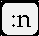
\includegraphics[width=18pt]{img/software_trans/2.pdf}} is given by node \code{:n} with non-terminal $n$ as node type and $out(S'):=$\raisebox{-.25\height}{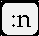
\includegraphics[width=18pt]{img/software_trans/2.pdf}},
    \item productions $P'$ and matches $M$ are given by $(P',M)=\mathcal{S}(\{(p,S')\},\varnothing)$ with $\mathcal{S}(H,MP'):=$ 
    $
    \begin{cases}
    \mathcal{S}(\{(p'',\ol{p}'') \mid (p'',\ol{p}'',\_,\_) \in MP''\},MP' \cup MP'') & ,\n{if }MP'' \neq \varnothing\\
    (\{\ol{p}'' \mid (\_,\ol{p}'',\_,\_) \in MP'\},\{\ol{m} \mid (\_,\_,\_,\ol{m}) \in MP'\}) & ,\n{otherwise}
    \end{cases}
	$
	\newline
	where $MP''=\{(p'',\ol{p}'',(l,n),\ol{m}) \mid (p\colon n \in N \to \_,\ol{p}) \in H,p''\colon n' \in N \to R'^* \in P,(l,n) \in R'^*,(p'',\_,(l,n),\_)\not\in MP'\} \cup \{(p'',\ol{p}'',(l,n),\ol{m}) \mid (p\colon n \in N \to \_,\ol{p}) \in H,p''\colon n' \in N \to R'^* \in P,(l,n) \in R'^*,(p'',\ol{p}'',(l,n),\_)\in MP',(p'',\ol{p}'',(l,n),\ol{m})\not\in MP'\}$
	with productions $\ol{p}'':=$\raisebox{-.25\height}{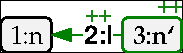
\includegraphics[width=80pt]{img/software_trans/1.pdf}} where $out(\ol{p}'')$ is given by node \code{3:n'} and matches $\ol{m}:=(1 \mapsto out(\ol{p}))$ with $s_{\GS_p}(\ol{m}):=\ol{p}''$ and $t_{\GS_p}(\ol{m}):=\ol{p}$
  \end{enumerate}
  Note that $G$ may contain several production rules with the same non-terminal $n \in N$ as LHS.
  The schemata for these production rules are combined in the sense that we construct the disjunction over the corresponding recursive graph constraints for $\ol{C}_G$.
\envEndMarker
\end{enumerate}
\end{definition}

An EBNF type graph together with a set of EBNF graph constraints form the meta-model for the graph language of derivation trees.
The elements of this language are called derivation graphs.

\begin{definition}[Derivation Graph]
\label{def:sec-compl-software-trans-mapping:der_graph}
\index{graph!derivation graph}
Let $G=(N,n_S,T,L,S,(C_s)_{s \in S},P)$ be an EBNF grammar with labels, $\TG_G^{DSIG}$ be the corresponding EBNF type graph and $C_G$ be the set of EBNF graph constraints w.r.t. $G$.
Then, \emph{a derivation graph} of $G$ is an attributed graph $DG=(\underline{DG},A)$ such that
\begin{enumerate}
  \item $DG$ is typed over $\TG_G^{DSIG}$,
  \item $DG$ satisfies the constraints $C_G$ ($DG \models C_G$), and
  \item $A$ is a $DSIG$-algebra with carrier sets $(C_s)_{s \in S}$.\envEndMarker
\end{enumerate}
\end{definition}

\begin{example}[Derivation Graph]
Note that the coding of EBNF grammars into EBNF type graphs in \cref{def:sec-compl-software-trans:ebnf_typegraph} neglects unlabelled terminals $T$ of the grammar to be part of derivation graphs whereas labelled terminals $(C_s)_{s \in S}$ may be contained in derivation graphs as node attribute values.
\cref{sec-compl-software-trans-tgg,fig:sec-compl-software-trans:ast} depicts a derivation graph of the EBNF grammar in \cref{ex:sec-compl-software-trans:ebnf} with the EBNF type graph in \cref{ex:sec-compl-software-trans-mapping:ebnf_tg} and corresponding EBNF graph constraints.
\envEndMarker
\end{example}

\begin{definition}[Graph Language of Derivation Trees]
\label{def:sec-compl-software-trans:graph_lang_der}
\index{language!graph language of derivation trees}
Let $G$ be an EBNF grammar with labels.
Then, \emph{the graph language $\Lang(G)$ of derivation trees of $G$} is given by all derivation graphs of $G$ according to \cref{def:sec-compl-software-trans-mapping:der_graph}.
\envEndMarker
\end{definition}

If all non-terminal in an EBNF grammar $G$ with labels are reachable from the start rule of the grammar, then the language of derivation trees of $G$ is isomorphic to the graph language of derivation trees of $G$, i.e., according to \cref{def:sec-compl-software-trans-prob:iso} there is a bijective mapping between both languages such that for each derivation tree over $G$ there is a corresponding graph in the graph language.
A non-terminal is reachable from the start rule in the grammar, if there is a path via from the start rule to the corresponding non-terminal which induces a derivation tree.
Note that for context-free grammars, the detection of unreachable non-terminals is decidable and their elimination terminates for grammars with a finite set of grammar rules, a finite set of non-terminals and where each grammar rule is finite (cf. Sec. 7.1.1. in \cite{DBLP:books/daglib/0011126}).

\begin{claim}[Isomorphism of Derivation Tree Languages]
\label{thm:sec-compl-software-trans:equ_lang_der}
Let $G$ be an EBNF grammar with labels such that all non-terminals are reachable from the start rule of the grammar.
Then, according to \cref{def:sec-compl-software-trans-prob:iso} the language $\Der(G)$ of derivation trees of $G$ and the graph language $\Lang(G)$ of derivation trees of $G$ are isomorphic.
\envEndMarker
\end{claim}